
\section{Results}\label{Sec:Results}

The results will be presented in two parts: First, the forecasting accuracy of the prediction models is evaluated and presented. Second, the results of the market simulation -- which is run once with the true consumption and production values and once with the predicted values -- are reported.


%%%%%%%%%%%%%%%%%%%%%%%%%%%%
%%%   Benchmark models   %%%
%%%%%%%%%%%%%%%%%%%%%%%%%%%%

\subsection{Evaluation of the prediction models}\label{Sec:Results;Subsec:Forecast}

Three prediction methods where used to forecast the energy consumption of 81 consumer data sets and to forecast the energy production of 12 prosumer data sets: a benchmark model (see Section~\ref{Sec:Method;Subsec:Benchmark}), a LSTM RNN model (see Section~\ref{Sec:Method;Subsec:LSTM}), and a LASSO model (see Section~\ref{Sec:Method;Subsec:LASSO}). All three prediction models were compared and evaluated using the error measures presented in Section~\ref{Sec:Method;Subsec:Error}.


%%%%%%%%%%%
\subsubsection{Consumption data}

The performance of the prediction models was tested on a quarter of the available data. That is, the prediction models were fitted on the consumption values from 01.01.2017~00:00 to 30.09.2017~00:00 which is equivalent to 131,040 data points per data set. For all 81 consumer data sets, the models were fitted separately resulting in as many distinct LASSO and LSTM prediction models. The fitted models were then used to make energy consumption predictions in 15-minute intervals for each household individually on the data from 01.10.2017~00:00 to 01.01.2018~00:00. This equates to 8,836 predicted values per data set per prediction method.

Figure~\ref{Fig:glimpse_predcons} exemplary shows the true and predicted consumption values of consumer 011 on October 27, 2017. The naive benchmark model just follows the true consumption shifted by one time step (i.e. 15 minutes). This fits the true values generally good, as long as there are no sudden jumps in the household's energy consumption. Spikes in energy consumption, as in this example one occurred in the 15 minutes before 07:30 and 08.30 respectively, necessarily lead to two periods with high errors of the naive predictor: First, once the jump to a high consumption level occurs and the naive predictor remains at the previous low level, and second, once the consumption suddenly returns to the low "baseline" consumption level and the naive predictor lags behind at the high level of the previous period. In such situations, the LASSO and LSTM models are more accurate. Even though, they underestimate the jumps in energy consumption, they do not lag behind as much as the naive predictor and, generally, have the ability to anticipate movements. However, the exemplary glimpse onto the predicted consumption values of consumer 011 already reveals that also the sophisticated prediction models lack the ability to accurately predict sudden movements in the energy consumption and tend to overestimate low consumption levels and underestimate spiking energy consumption.
%
\begin{figure}[htbp]
    \centering
    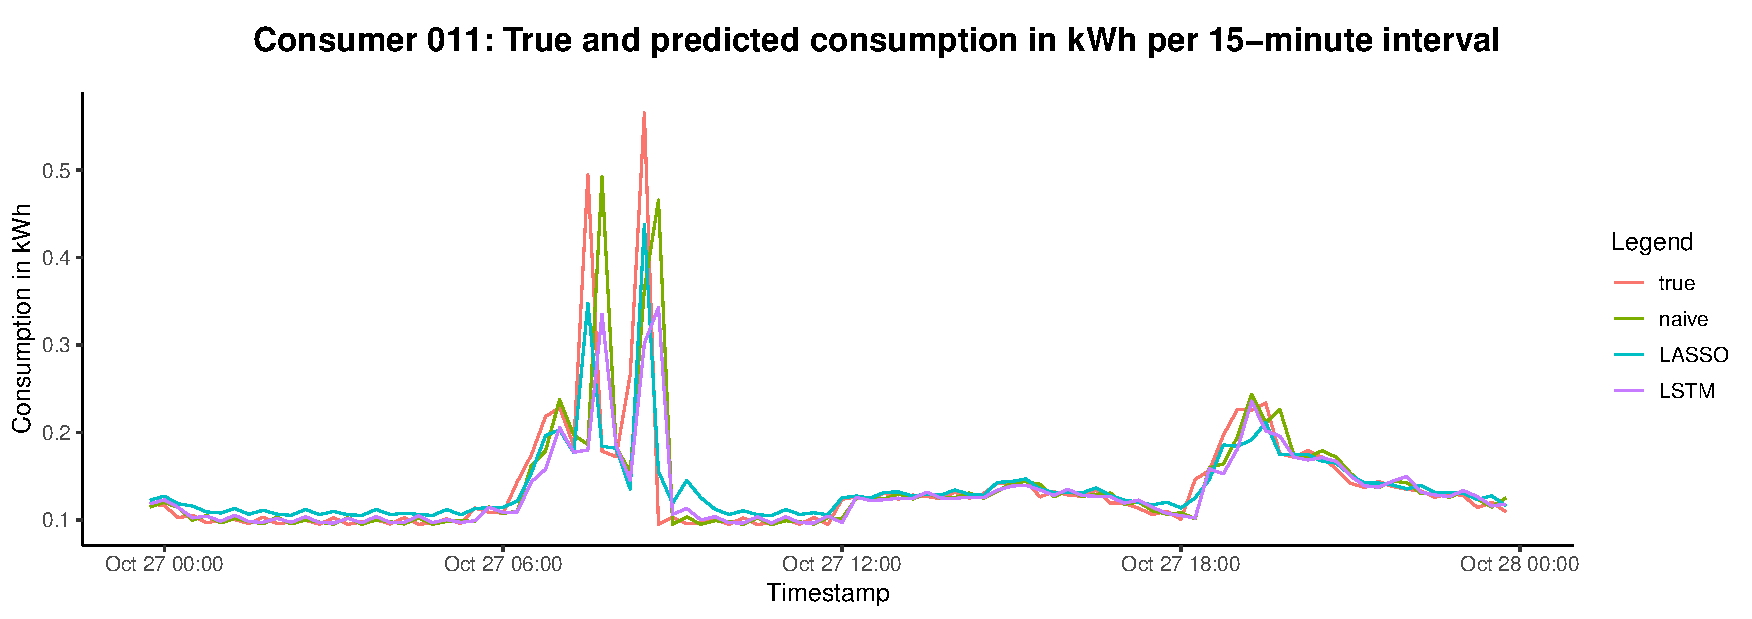
\includegraphics[width=\textwidth]{thesis/graphs/evaluation/c011_pred_cons.pdf}
    \caption[Exemplary 24 hours of true and predicted consumption values]{Exemplary 24 hours of true and predicted consumption values of consumer 011. \quantnet\href{}{}}
    \label{Fig:glimpse_predcons}
\end{figure}
%

Systematically analyzing the total over- and underestimation of the different prediction models on each consumer data set confirms this impression. Figure~\ref{Fig:overunderestimation} displays the total sum of over- and underestimation errors of each prediction method per data set. As one would expect, the naive benchmark model consistently over- and underestimated by the same amount per data set. The reason for that is, that the sum of over- and underestimation errors only depends on the amplitude of the jumps in the case of the naive predictor. Thus, overestimation errors occur in the same frequency and magnitude as underestimation errors. The LASSO model achieved overall lower total sums of errors than the benchmark model. Moreover, the sum of underestimation errors is higher across the data sets than the sum of overestimation errors. This points towards a general tendency of underestimating sudden increases in energy consumption by the LASSO model. The LSTM model on the other hand shows a much higher variability in the sum of over- and underestimation errors. By tendency, the overestimation errors of the LSTM model were smaller than those of the LASSO and benchmark models. Nevertheless, the underestimation is much more pronounced in the case of the LSTM model. Especially, some data sets stand out regarding the high sum of underestimation errors. This points towards a much higher heterogeneity in the suitability of the LSTM model to predict consumption values depending on the energy consumption pattern of the specific data set. The LASSO model on the other hand seems to be more equally well suited for all data sets and their particular consumption patterns.
%
\begin{figure}
    \centering
    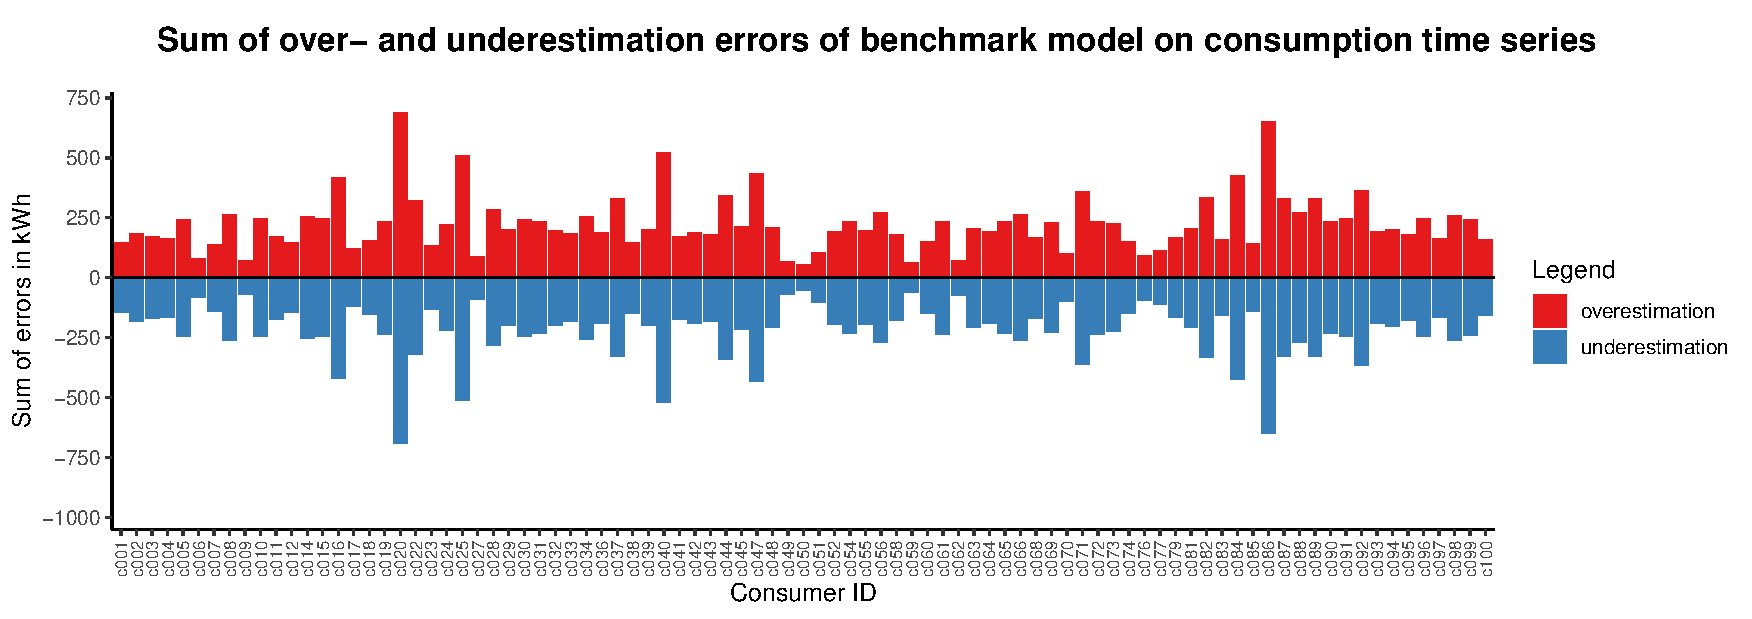
\includegraphics[width=\textwidth]{thesis/graphs/evaluation/c_barplot_naive_overunderestimation.pdf}\\\vspace{.6cm}
    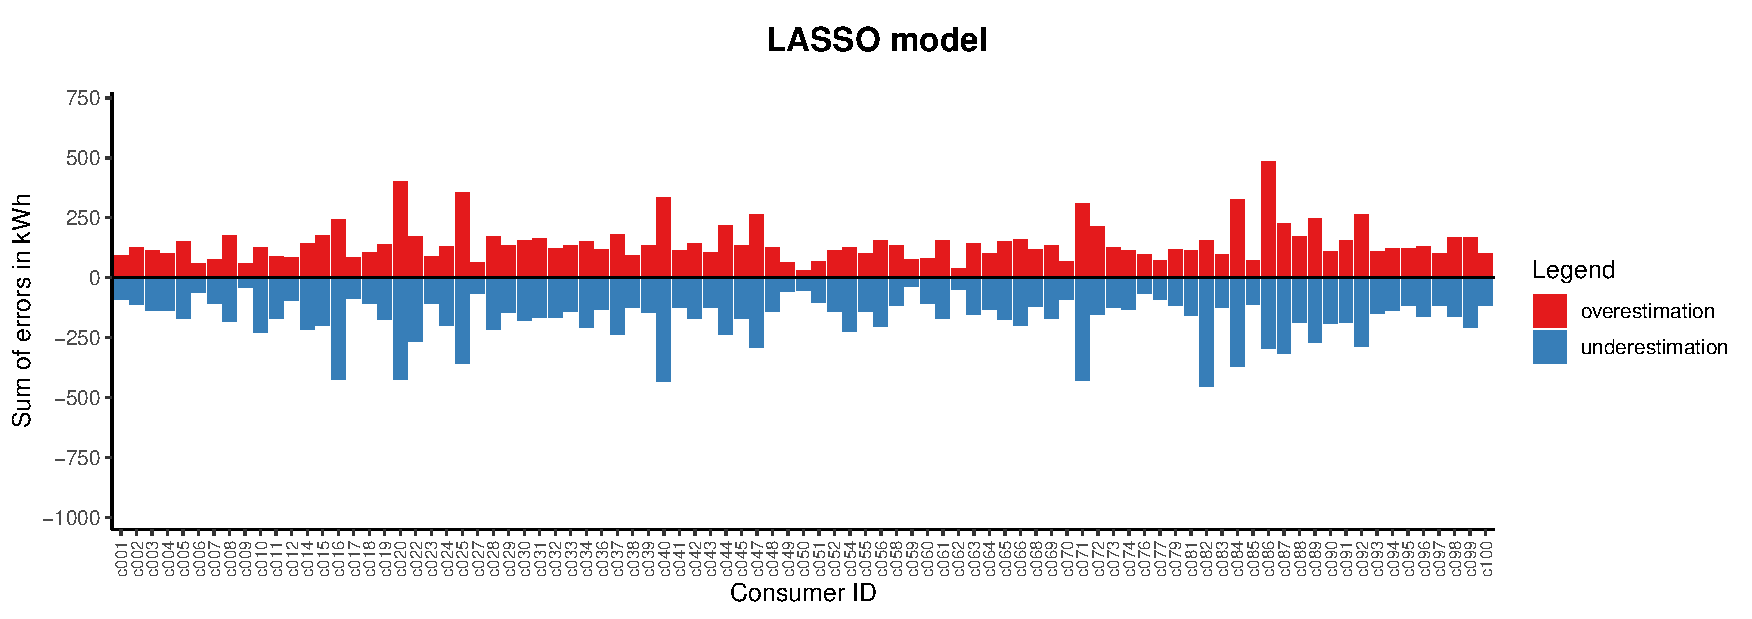
\includegraphics[width=\textwidth]{thesis/graphs/evaluation/c_barplot_LASSO_overunderestimation.pdf}\\\vspace{.6cm}
    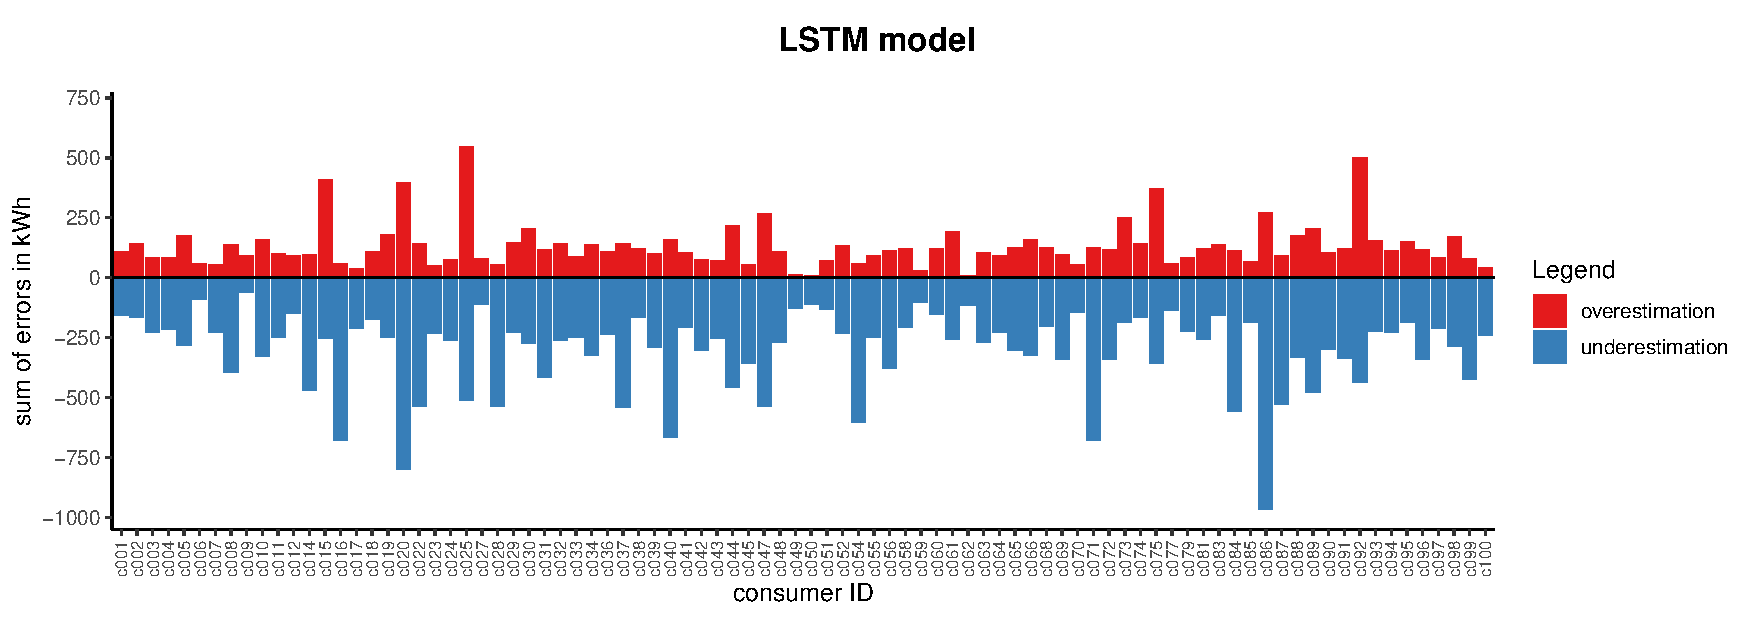
\includegraphics[width=\textwidth]{thesis/graphs/evaluation/c_barplot_LSTM_overunderestimation.pdf}
    \caption[Sum of total over- and underestimation errors per data set]{Sum of total over- and underestimation errors per data set and prediction model. \quantnet\href{}{}}
    \label{Fig:overunderestimation}
\end{figure}
%

The average performance of the three prediction models across all 81 data sets is shown in Table~\ref{Tab:avg_errormeasures}. As can be seen, LASSO and LSTM outperform the benchmark model according to MAE, RMSE, MAPE, and MASE by around 10 \%. Interestingly, due to the heavy penalty NRMSE puts on comparably large prediction errors, both sophisticated prediction methods perform worse according to NRMSE. A detailed analysis, however, reveals that this result is mainly driven, by one extremely bad NRMSE score for LSTM and LASSO on merely one out of the 81 data sets. As can be seen in Figure~\ref{Fig:heatmaps}, the predictions on consumer data set 027 have a particularly high NRMSE compared to all other data sets. However, this pattern is not present when using RMSE as error measure.\footnote{Note, that the MASE score of the benchmark model must be exactly one as the MASE is defined as the mean absolute error absolute to the MAE of the naive predictor (see Equation~\ref{Eq:naivepred}).}
%
\begingroup\catcode`"=9
\begin{table}[ht]
{\footnotesize
    \csvreader[centered tabular=l|SSSSS,
    before reading=\sisetup{round-mode=places,round-precision=2,round-integer-to-decimal},
    filter not strcmp={\thecsvinputline}{1},
    table head=
    \hline\hline
     \multicolumn{1} {l}{\textbf{Model}} & \multicolumn{1} {|c}{\textbf{MAE}} & \multicolumn{1} {c}{\textbf{RMSE}} & \multicolumn{1} {c}{\textbf{MAPE}} & \multicolumn{1} {c}{\textbf{NRMSE}} & \multicolumn{1} {c}{\textbf{MASE}}\\
    \hline,
    no head,
    separator=comma,
    respect all,
    late after line=\\,
    table foot=\hline \hline]
    {thesis/tables/avg_errorMeasures.csv}{}%
    {\csvcolii & \csvcoliii & \csvcoliv & \csvcolv & \csvcolvi & \csvcolvii}}%
    \caption[Mean of error measures for all 82 consumer data sets]{Mean of error measures for the prediction of energy consumption across all 82 consumer data sets. \quantnet\href{ }{}}
    \label{Tab:avg_errormeasures}
\end{table}
\endgroup
%
%
\begingroup\catcode`"=9
\begin{table}[ht]
{\footnotesize
    \csvreader[centered tabular=l|SSSSS,
    before reading=\sisetup{round-mode=places,round-precision=2,round-integer-to-decimal},
    filter not strcmp={\thecsvinputline}{1},
    table head=
    \hline\hline
     \multicolumn{1} {l}{\textbf{Model}} & \multicolumn{1} {|c}{\textbf{MAE}} & \multicolumn{1} {c}{\textbf{RMSE}} & \multicolumn{1} {c}{\textbf{MAPE}} & \multicolumn{1} {c}{\textbf{NRMSE}} & \multicolumn{1} {c}{\textbf{MASE}}\\
    \hline,
    no head,
    separator=comma,
    respect all,
    late after line=\\,
    table foot=\hline \hline]
    {thesis/tables/median_errorMeasures.csv}{}%
    {\csvcolii & \csvcoliii & \csvcoliv & \csvcolv & \csvcolvi & \csvcolvii}}%
    \caption[Median of error measures for all 82 consumer data sets]{Median of error measures for the prediction of energy consumption across all 82 consumer data sets. \quantnet\href{ }{}}
    \label{Tab:avg_errormeasures}
\end{table}
\endgroup
%
%
\begingroup\catcode`"=9
\begin{table}[ht]
{\footnotesize
    \csvreader[centered tabular=l|SSSSSSS,
    before reading=\sisetup{round-mode=places,round-precision=2,round-integer-to-decimal},
    filter not strcmp={\thecsvinputline}{1},
    table head=
    \hline\hline
     \multicolumn{1} {l}{\textbf{Model}} & \multicolumn{1} {|c}{\textbf{MAE}} & \multicolumn{1} {c}{\textbf{RMSE}} & \multicolumn{1} {c}{\textbf{MAPE}} & \multicolumn{1} {c}{\textbf{MdAPE}} & \multicolumn{1} {c}{\textbf{NRMSE}} & \multicolumn{1} {c}{\textbf{NRMdSE}} & \multicolumn{1} {c}{\textbf{MASE}}\\
    \hline,
    no head,
    separator=comma,
    respect all,
    late after line=\\,
    table foot=\hline \hline]
    {thesis/tables/avg_errorMeasures_corrected.csv}{}%
    {\csvcolii & \csvcoliii & \csvcoliv & \csvcolv & \csvcolvi & \csvcolvii & \csvcolviii & \csvcolix}}%
    \caption[Mean of error measures across all 82 consumer data sets]{Mean of error measures for the prediction of energy consumption across all 82 consumer data sets including the median absolute percentage error (MdAPE) and normalized root median squared error (NRMdSE). \quantnet\href{ }{}}
    \label{Tab:avg_errormeasures}
\end{table}
\endgroup
%
%
\begin{figure}[htbp]
 \centering
 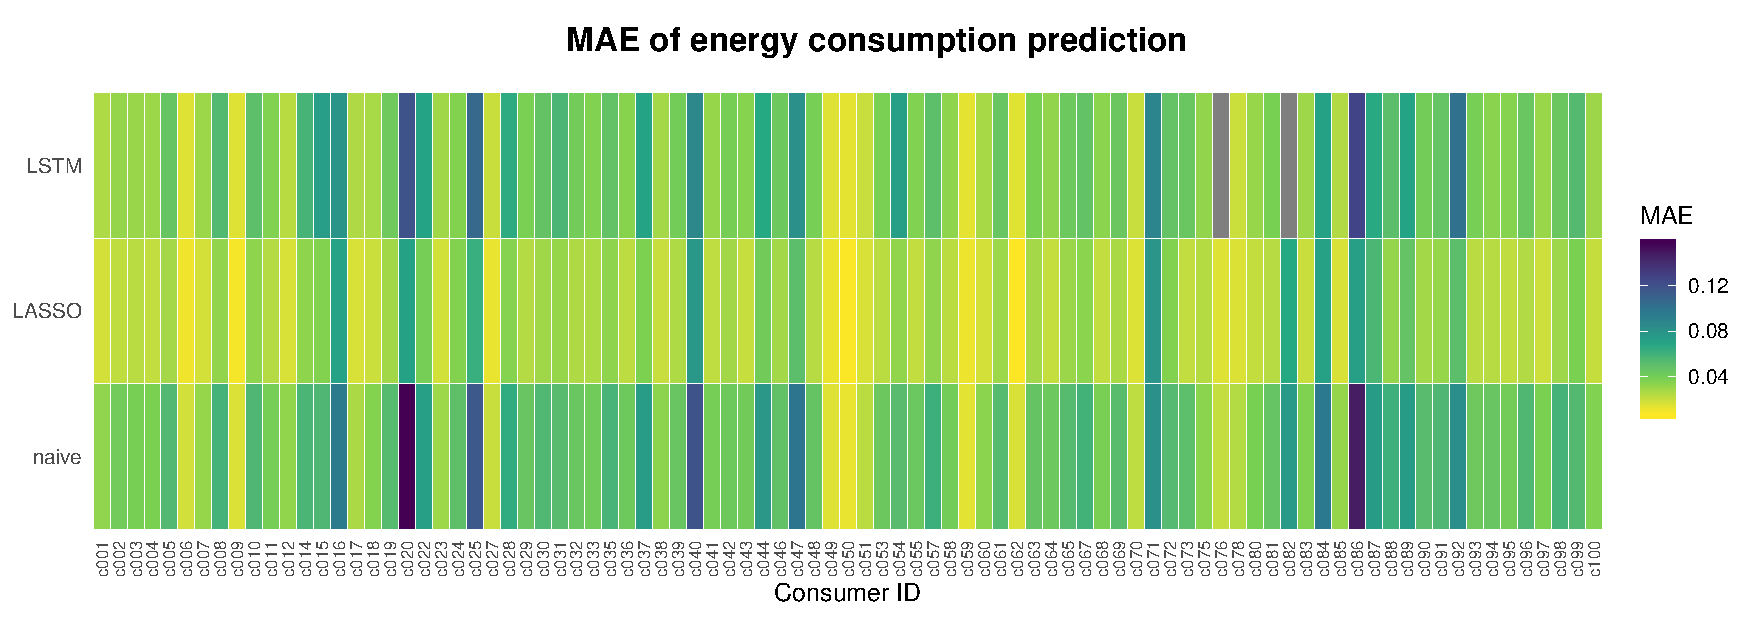
\includegraphics[width=\textwidth]{thesis/graphs/evaluation/c_heatmap_MAE.pdf}
 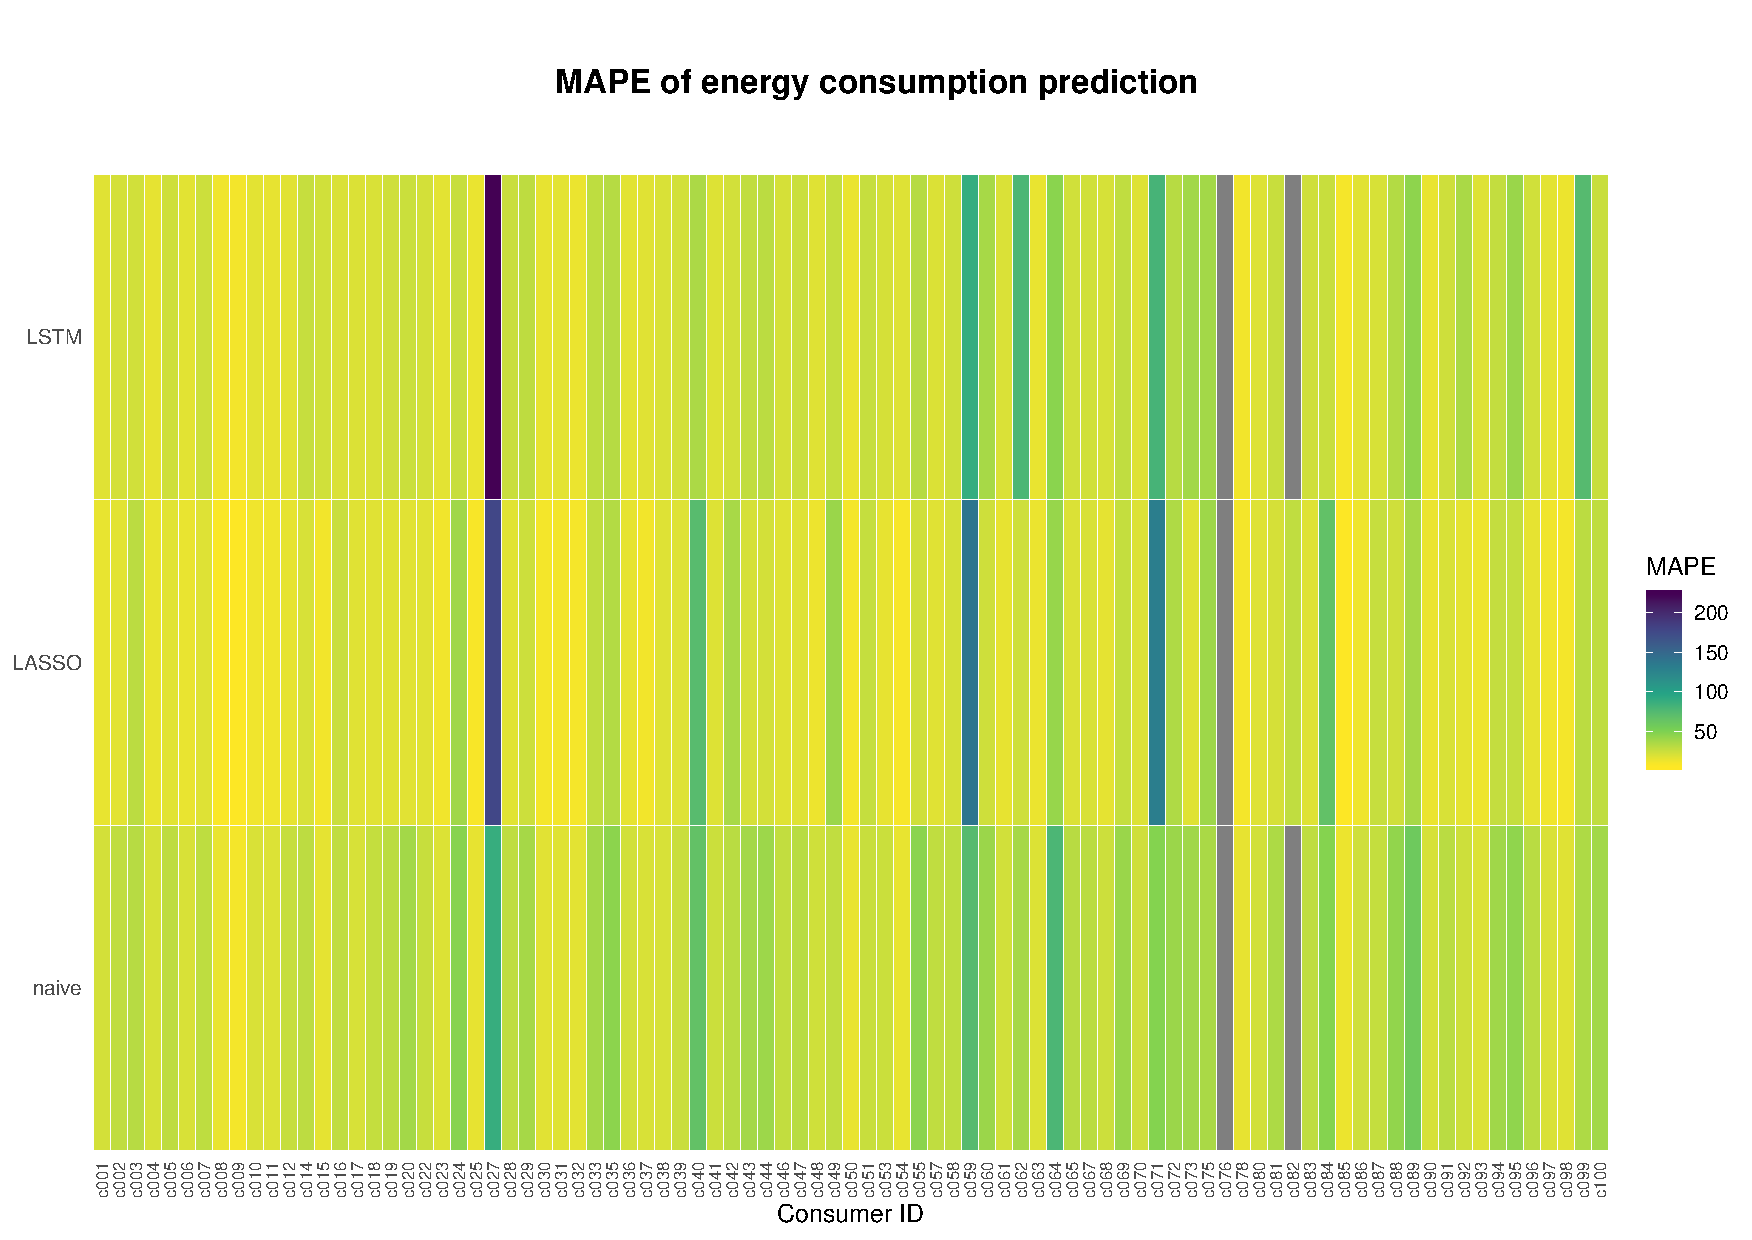
\includegraphics[width=\textwidth]{thesis/graphs/evaluation/c_heatmap_MAPE.pdf}
 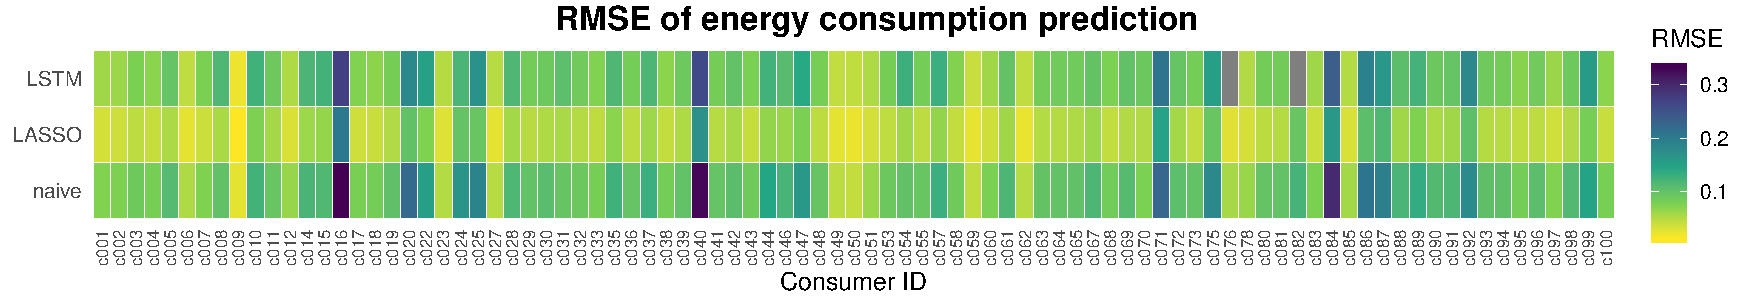
\includegraphics[width=\textwidth]{thesis/graphs/evaluation/c_heatmap_RMSE.pdf}
 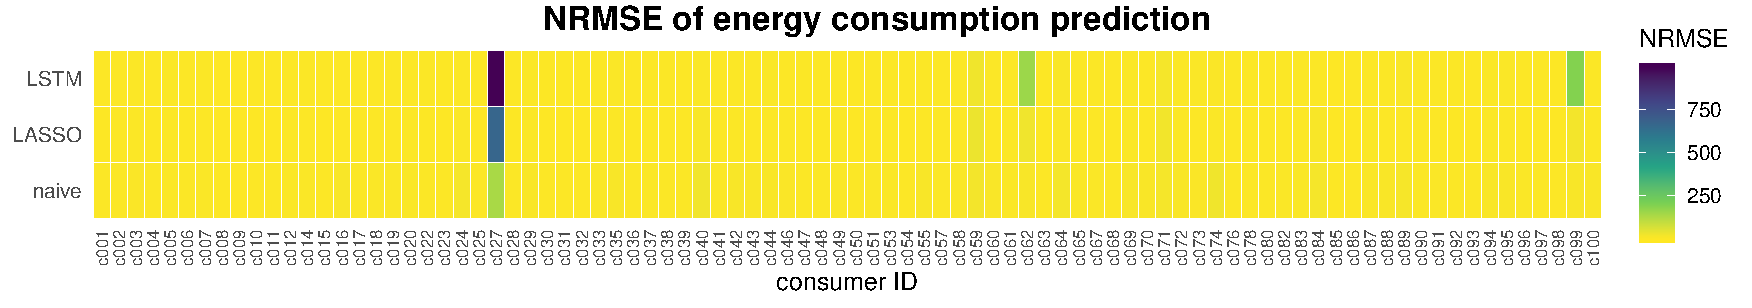
\includegraphics[width=\textwidth]{thesis/graphs/evaluation/c_heatmap_NRMSE.pdf}
 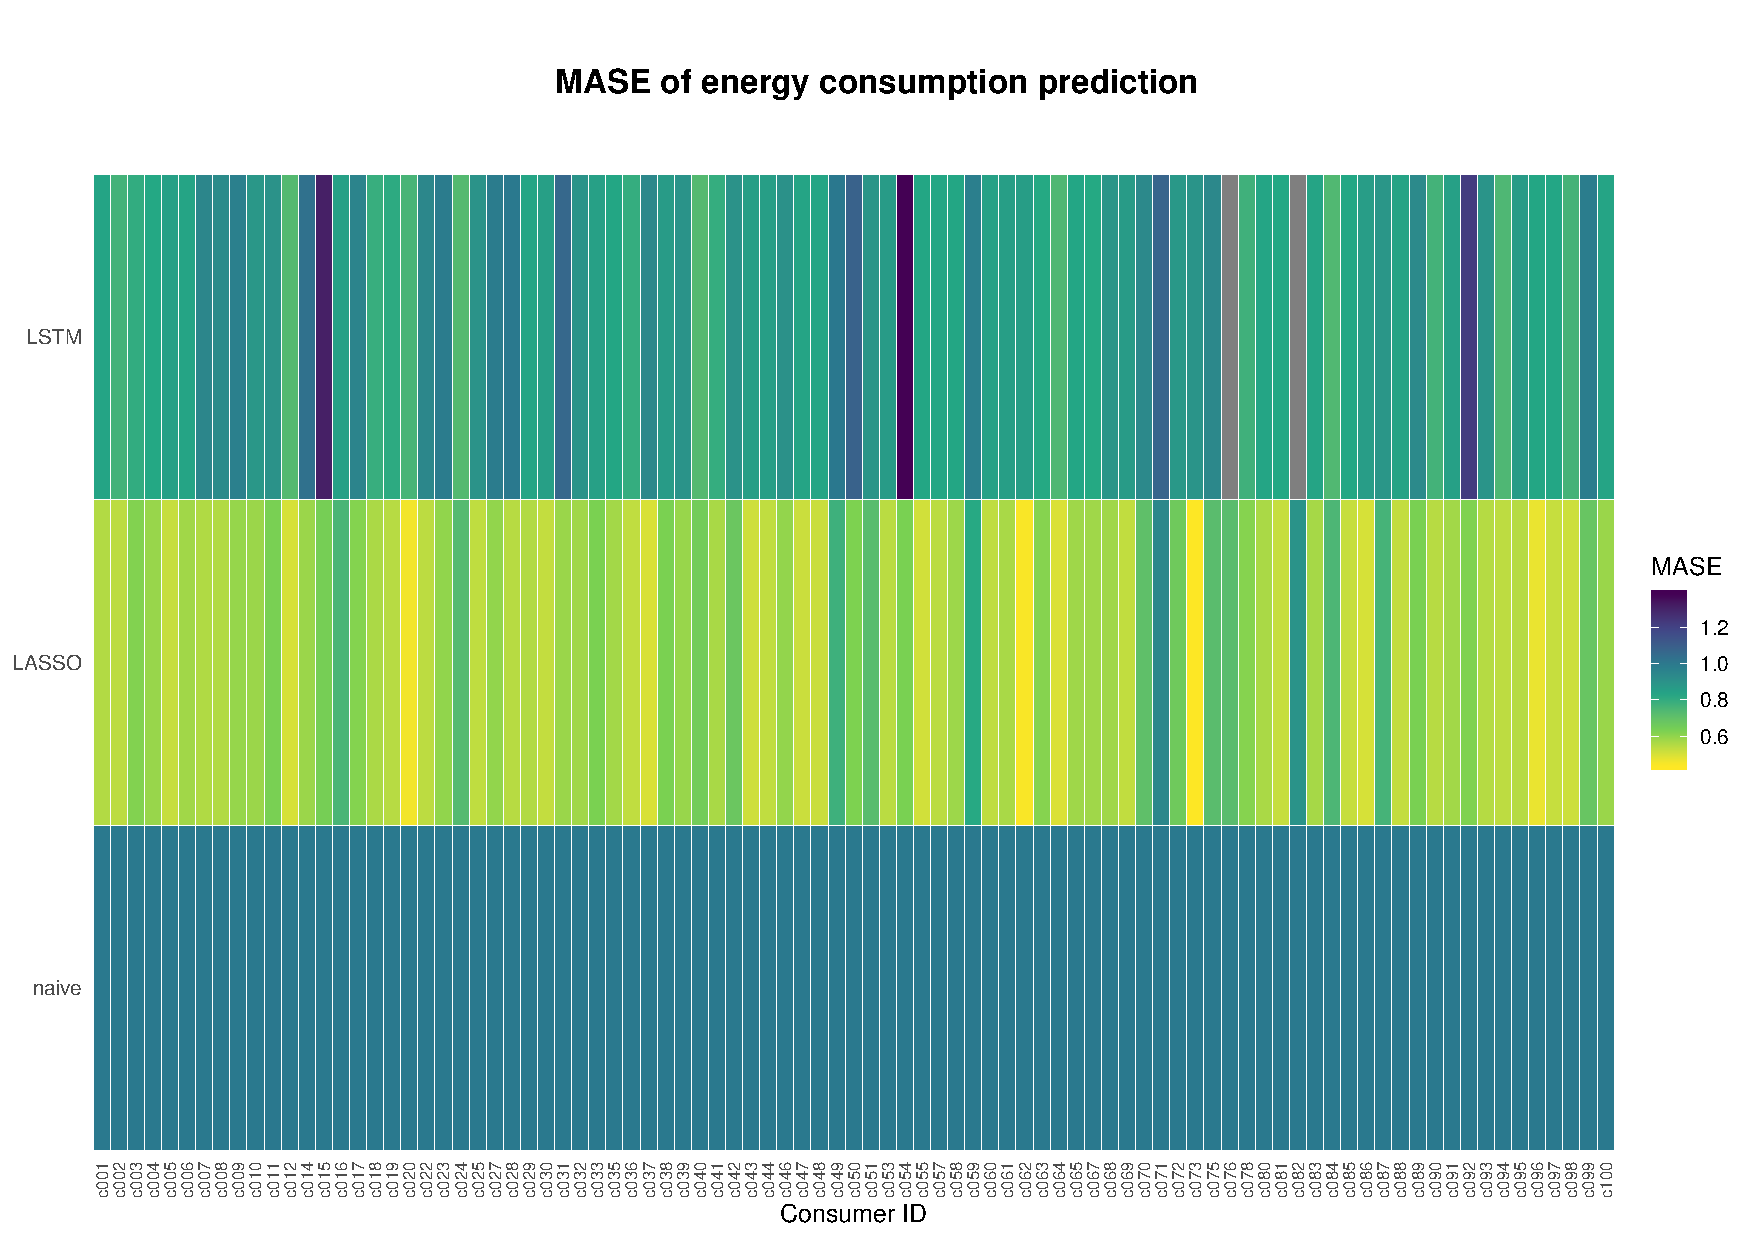
\includegraphics[width=\textwidth]{thesis/graphs/evaluation/c_heatmap_MASE.pdf}
\caption[Heatmaps of all error measures for consumption values]{Heatmap of MAE, MAPE, RMSE, NRMSE, and MASE scores for the prediction of consumption values per consumer data set. \quantnet\href{ }{}}
\label{Fig:heatmaps}
\end{figure}
%

Further investigating the prediction errors of the forecasts on consumer 026 exposes that the high NRMSE score is driven by merely one observations: Between 24.11.2017 11:30 and 11:45 the energy consumption falls below 3 $\times$ $10^{-6}$. Due to this, the relative squared error $e_t = \left(\frac{\widehat{x}_t-x_t}{x_t}\right)^2$ explodes (see Appendix~\hyperlink{AppA4:Figures:erroranalysis}{A4}). This single extreme error pushes the NRMSE of the LSTM predictions to the staggering value of 2383.46 while the normalized root \emph{median} squared error is only 33.43 (which is still comparatively high). The same is true for MAPE, though not as extreme.

Overall, the LASSO model performed best with the lowest MAE, RMSE, MAPE, and MASE scores. However, with a MAPE of 24.43 \%, it achieved a worse score in this study than in the implementation of \citet{Li:2017}, who achieved a score of 20.06 \%. The superior performance of the LASSO model is also clearly visible in Figure~\ref{Fig:boxplots_errormeasures}. Additionally noteworthy here is the differences in the IQR of the error measures between the prediction methods. Both, the LASSO as well as the LSTM model, have error measures with a smaller IQR across the consumer data sets than the benchmark model. Furthermore, even though the LASSO error measures consistently have the lowest median of all three prediction models, the IQR of the relative error measures MAPE and NRMSE is very similar between LASSO and LSTM.

Interestingly, there are some consumer data sets with apparently much harder to predict consumption patterns than the other data sets which becomes visible by the outliers of the MAPE and NRMSE boxplots but also by the heatmaps displayed in Figure~\ref{Fig:heatmaps}. They grey fields in the heatmaps of consumer 076 and 082 indicate missing values for the respective error measures and are introduced by zero consumption values that are present in the data of those consumers. As can be seen in Equation~\ref{Eq:MAPE} and Equation~\ref{Eq:NRMSE}, MAPE and NRMSE are not defined if the true value $x_t$ equals zero which is why they cannot be computed for consumer 076 and 082.


%
\begin{figure}
    \centering
    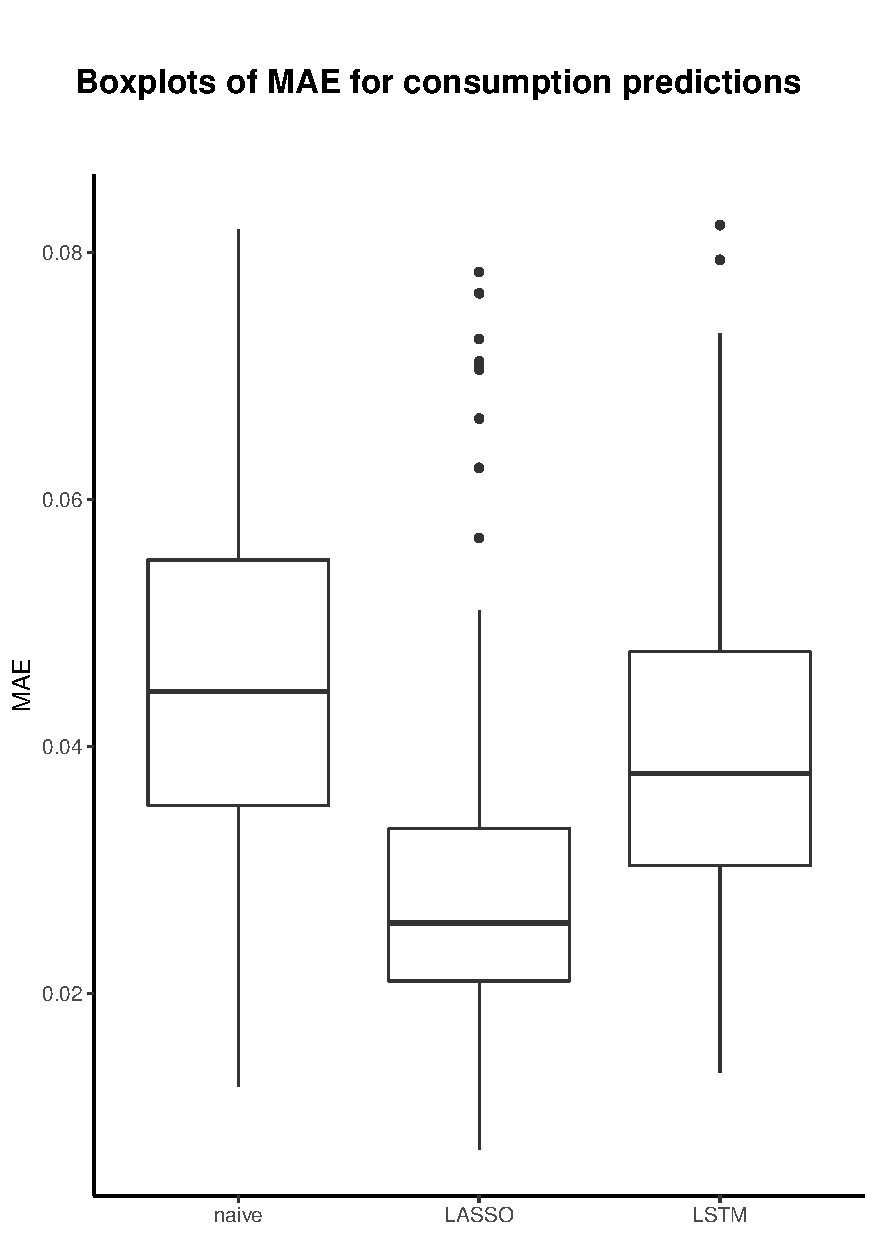
\includegraphics[width=.5\textwidth-5pt]{thesis/graphs/evaluation/c_boxplot_MAE.pdf}
    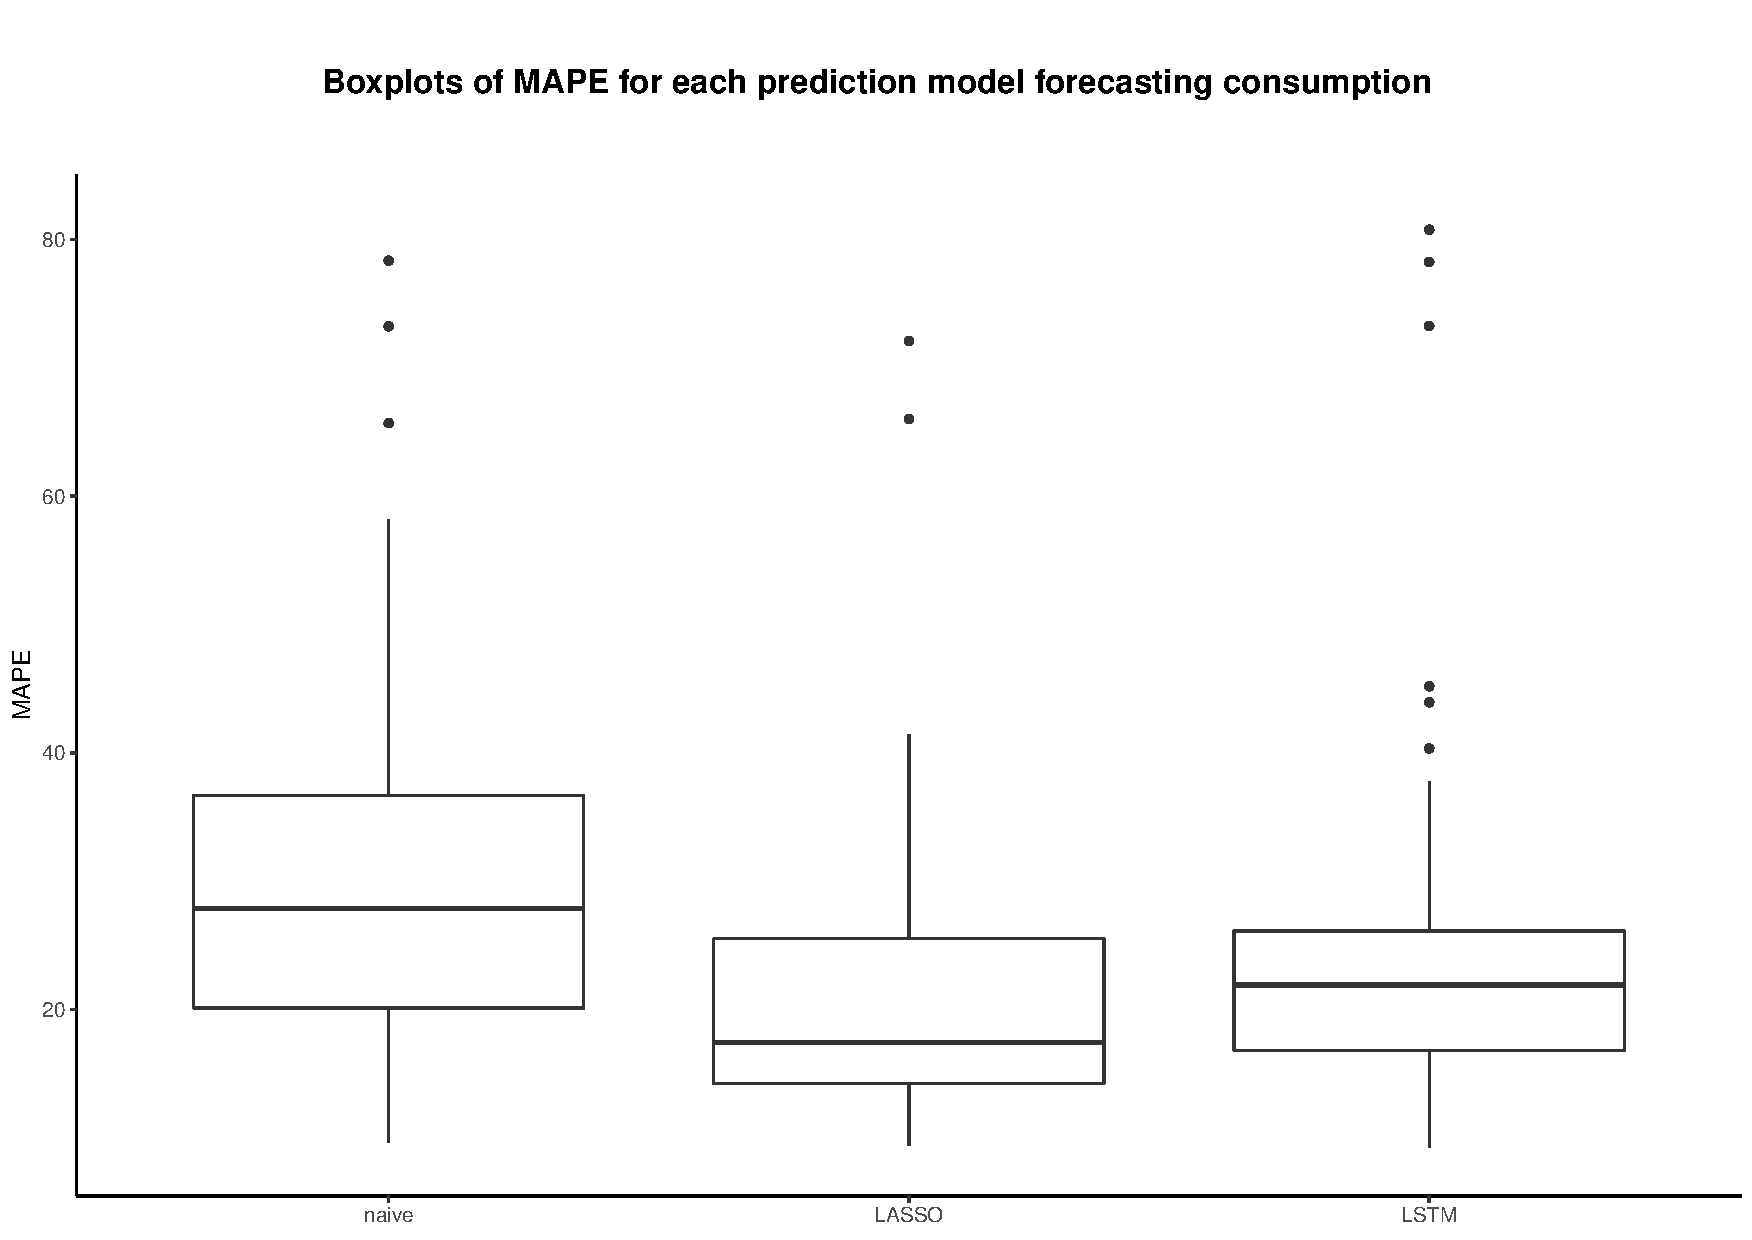
\includegraphics[width=.5\textwidth-5pt]{thesis/graphs/evaluation/c_boxplot_MAPE.pdf} \\
    
    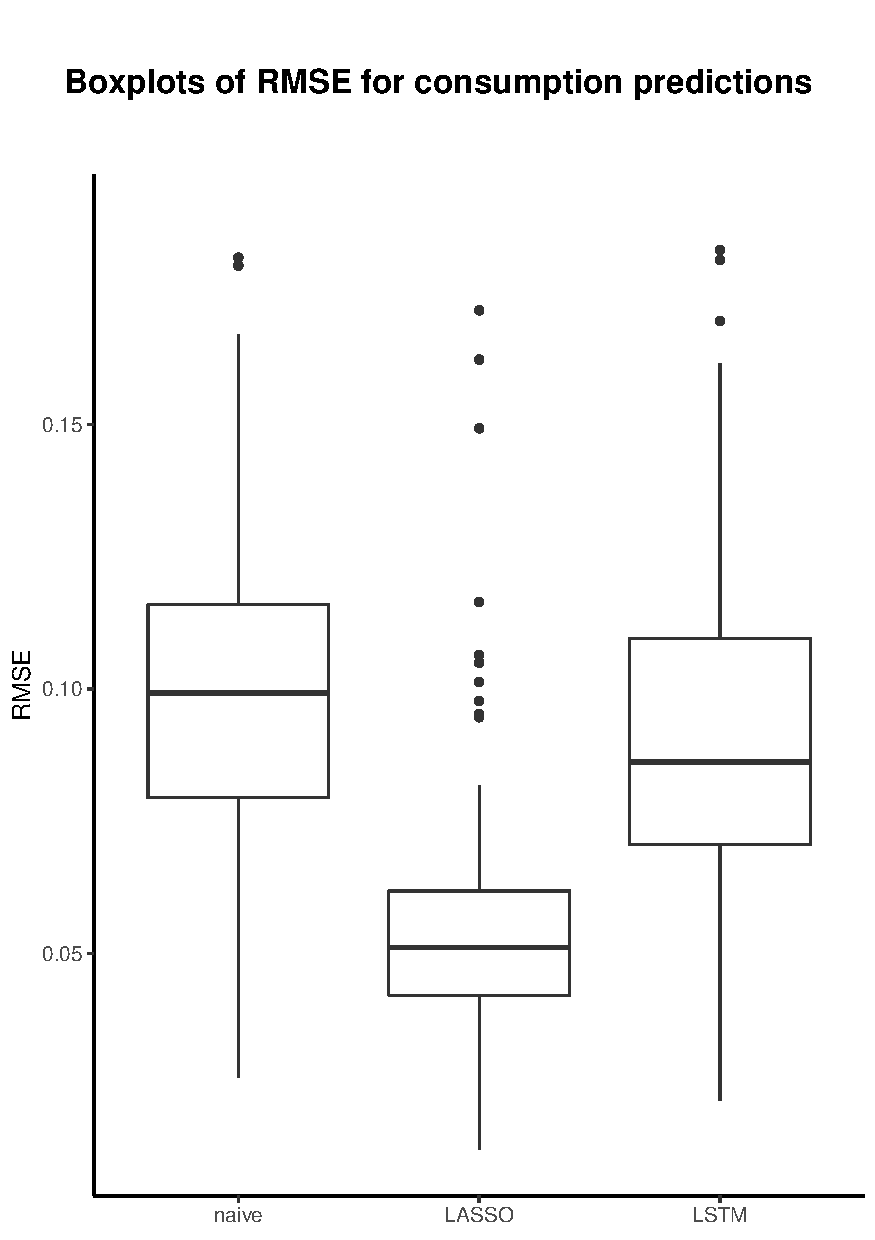
\includegraphics[width=.5\textwidth-5pt]{thesis/graphs/evaluation/c_boxplot_RMSE.pdf}
    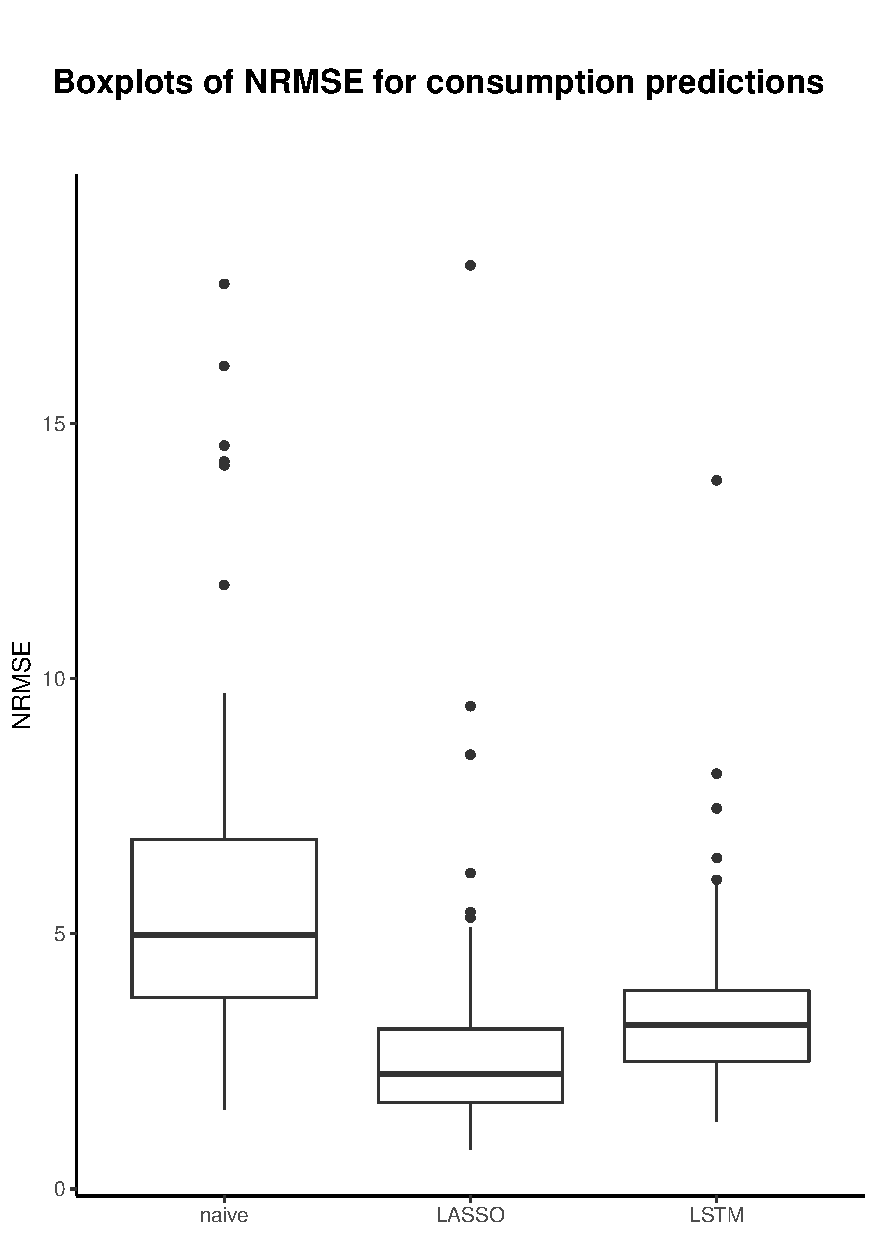
\includegraphics[width=.5\textwidth-5pt]{thesis/graphs/evaluation/c_boxplot_NRMSE.pdf} \\
    \caption[Boxplots of MAE, MAPE, RMSE, and NRMSE scores across 82 consumer data sets]{Boxplots of MAE, MAPE, RMSE, and NRMSE scores across 82 consumer data sets for the three different prediction models (the upper 3 \%-quantile of the error measures is cut off for better readability). \quantnet\href{}{}}
    \label{Fig:boxplots_errormeasures}
\end{figure}


%%%%%%%%%%%
\subsubsection{Production data}



%%%%%%%%%%%%%%%%%%%%%%%%%%%%
%%%   Market simulation   %%%
%%%%%%%%%%%%%%%%%%%%%%%%%%%%

\subsection{Evaluation of the market simulation}\label{Sec:Results;Subsec:Simulation}



%%%%%%%%%%%
\subsubsection{True consumption and production values}



%%%%%%%%%%%
\subsubsection{Predicted consumption and production values}



%%%%%%%%%%%
\subsubsection{Cost due to prediction errors}



%%%%%%%%%%%%%%%%%%%%%%%%%%%%%%%%%%%%%%%%%%%%%%%%%%%%%%%%%%%%%%%%%

\begin{itemize}

    \item Organize material and present results.

    \item Use tables, figures (but prefer visual presentation):
        \begin{itemize}
            \item Tables and figures should supplement (and not duplicate) the
                text.

            \item Tables and figures should be provided with
            legends.\\
                {\it Figure~\ref{Fig:Resids} shows how to include and reference
                graphics. The graphic must be labelled before. Files must be in
                \texttt{.eps} format.}

                \begin{figure}[ht]
                \begin{center}
                    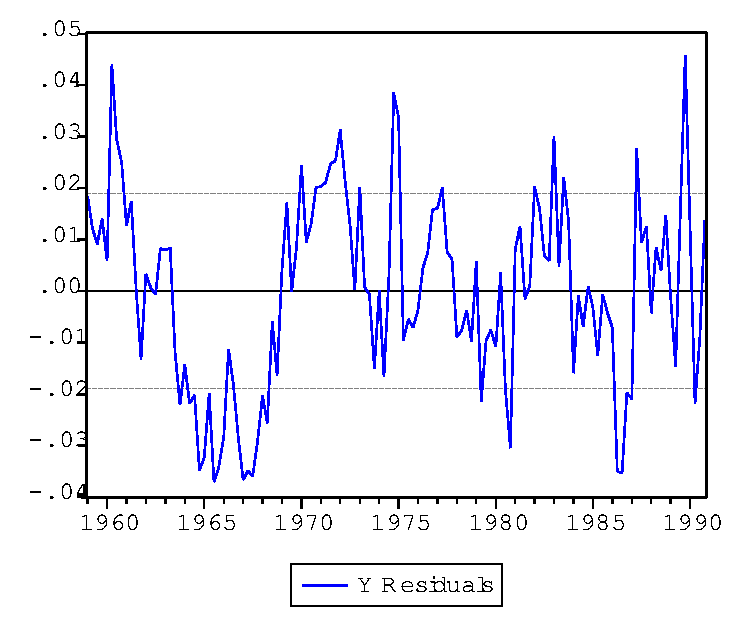
\includegraphics[scale=0.5,angle=0]{thesis/figures/graph.pdf}
                    \caption{Estimated residuals from model XXX. ...}
                    \label{Fig:Resids}
                \end{center}
                \end{figure}

            \item Tables and graphics may appear in the text or in
                the appendix, especially if there are many simulation results
                tabulated, but is also depends on the study and number of tables resp.
                figures. The key graphs and tables must appear in
                the text!
        \end{itemize}

    \item Latex is really good at rendering formulas:\\
        {\it Equation (\ref{Eq:SpecDens}) represents the ACs of a stationary
        stochastic process:
        \begin{equation}
            f_y(\lambda) = (2\pi)^{-1} \sum_{j=-\infty}^{\infty}
                           \gamma_j e^{-i\lambda j}
                         =(2\pi)^{-1}\left(\gamma_0 + 2 \sum_{j=1}^{\infty}
        \gamma_j \cos(\lambda j)\right)
                                        \label{Eq:SpecDens}
        \end{equation}
        where $i=\sqrt{-1}$ is the imaginary unit, $\lambda \in [-\pi,
        \pi]$ is the frequency and the $\gamma_j$ are the autocovariances
        of $y_t$.}

\newpage

    \item Discuss results:
        \begin{itemize}
            \item Do the results support or do they contradict economic theory ?
            \item What does the reader learn from the results?
            \item Try to give an intuition for your results.
            \item Provide robustness checks.
            \item Compare to previous research.
        \end{itemize}
\end{itemize}
